\documentclass{article}
\usepackage{changepage}
\usepackage{graphicx}
\usepackage{float}

\title{IN618 - Assignment 1}
\author{Matthew Hall}
\date{}

\begin{document}
\pagenumbering{gobble}
\maketitle
\newpage
\pagenumbering{arabic}

\tableofcontents
\newpage

\section{Host Discovery}

\subsection{Discovering hosts with nmap}
\paragraph{}
I used the following commands during the host discorvery process:

\texttt{nmap -sn 192.168.100.1}

The above command identifies hosts with IP addresses in the network space of 192.168.100.0/24

\texttt{nmap -O 192.168.100.1}

The above command attempts to identify the operating system of the host with address 192.168.100.1

\texttt{nmap -O 192.168.100.115}

The above command attempts to identify the operating system of the host with address 192.168.100.115

\texttt{nmap -O 192.168.100.253}

The above command attempts to identify the operating system of the host with address 192.168.100.253

\subsection{Network Diagram}

\begin{figure}[h!]
	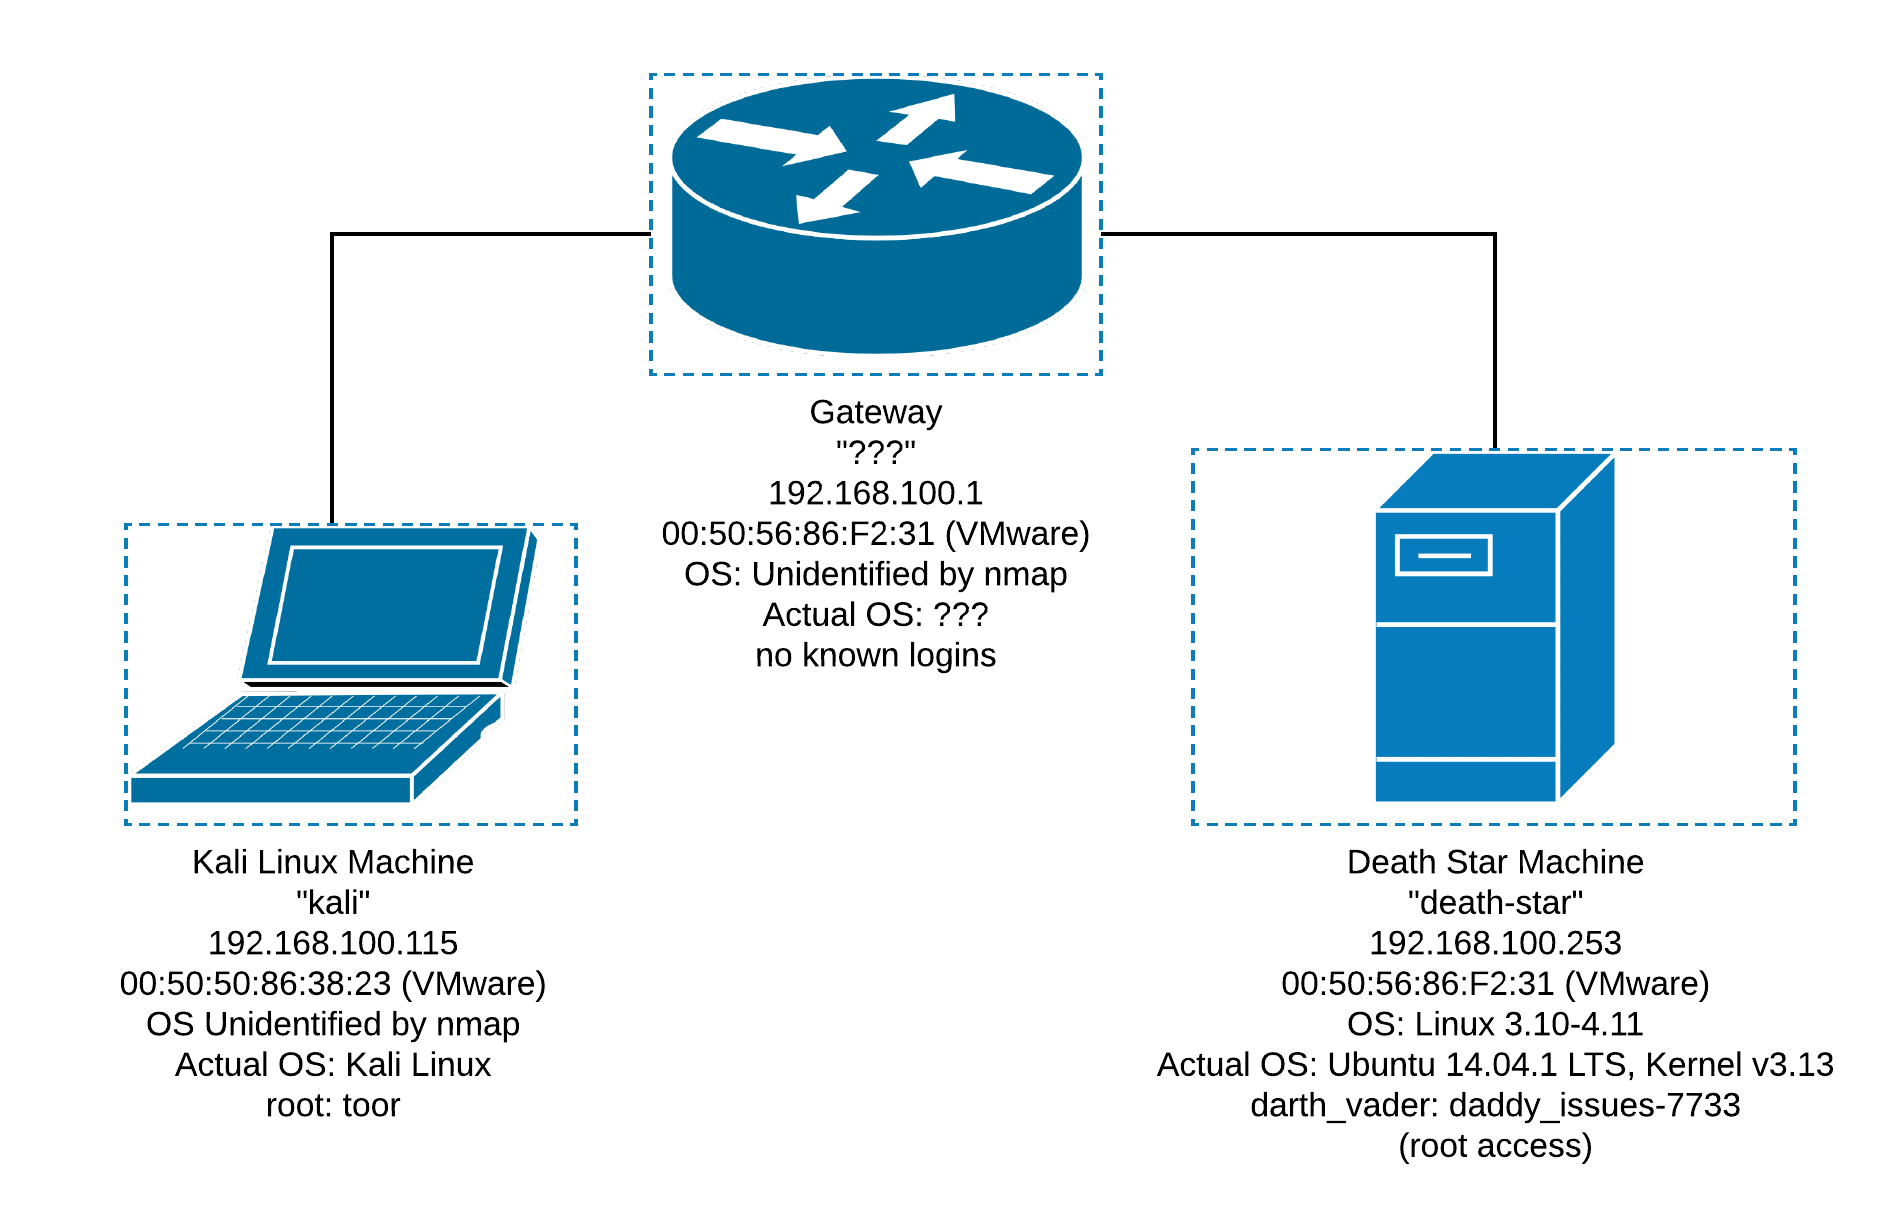
\includegraphics[width=\linewidth]{resources/network-diagram.png}
	\caption{Network diagram of address space \texttt{192.168.100.0/24}}
	\label{fig:network-diagram}
\end{figure}

\newpage

\section{Information Gathering}
\paragraph{}
By use of the nmap command \texttt{nmap -sV 192.168.100.253}, I was able to retrieve the following information about what services on the target machine are running on what ports:
\newline
\newline

\begin{adjustwidth}{-2cm}{}
\begin{tabular}{ |c|c|c|l| }
\hline
Port Number & State & Service & Version \\
\hline
21/tcp & open & ftp & ProFTPD 1.3.5 \\
\hline
22/tcp & open & ssh & OpenSSH 6.6.1p1 Ubuntu 2ubuntu2.10 (Ubuntu Linux; protocol 2.0) \\
\hline
80/tcp & open & http & Apache httpd 2.4.7 \\
\hline
111/tcp & open & rpcbind & 2-4 (RPC \# 100000) \\
\hline
139/tcp & open & netbios-ssn & Samba smbd 3.X - 4.X (workgroup: WORKGROUP) \\
\hline
445/tcp & open & netbios-ssn & Samba smbd 3.X - 4.X (workgroup: WORKGROUP) \\
\hline
3306/tcp & open & mysql & MySQL (unauthorized) \\
\hline
6667/tcp & open & irc & UnrealIRCd \\
\hline
6697/tcp & open & irc & UnrealIRCd \\
\hline
8067/tcp & open & irc & UnrealIRCd \\
\hline
8080/tcp & open & http & Jetty 8.1.7.v20120910 \\
\hline
8181/tcp & open & http & WEBrick httpd 1.3.1 (Ruby 2.3.6 (2017-12-14)) \\
\hline
49307/tcp & open & status & 1 (RPC \# 100024) \\
\hline
\end{tabular}
\end{adjustwidth}

\newpage

\section{Vulnerability Identification}
\paragraph{}
The following services on the target machine had exploitable vulnerabilities:

% Port 21/tcp
\subsection{ProFTPD 1.3.5}
\paragraph{}
Version 1.3.5 of ProFTPD has vulnerability \emph{CVE-2015-3306}, which allows attackers to read and write to arbitrary files via the \texttt{site cpfr} and \texttt{site cpto} commands.\footnote{https://cve.mitre.org/cgi-bin/cvename.cgi?name=CVE-2015-3306}
Metasploit has the module \texttt{exploit/unix/ftp/proftpd\_modcopy\_exec} which exploits this flaw.
By using this module and specifying the \texttt{SITEPATH} option to be \texttt{/var/www/html}, I was able to remotely log in to the machine as the \texttt{www-data} user.
While logged in, I was able to download files in the \texttt{/var/www/html} directory\footnote{Among those files was the administrator account details of the phpMyAdmin service} and traverse the rest of the filesystem after starting an interactive shell.

% Ports 6667/tcp, 6697/tcp and 8067/tcp
\subsection{UnrealIRCd 3.2.8.1}
\paragraph{}
During the period of time from November 2009 to June 2010, version 3.2.8.1 of UnrealIRCd contained \emph{CVE-2010-2075}: a backdoor allowing remote attackers to login to the system and execute arbitrary commands.\footnote{https://cve.mitre.org/cgi-bin/cvename.cgi?name=CVE-2010-2075}
This vulnerability was only present in copies of the software downloaded from particular mirror sites.
This backdoor, if present, can be exploited with metasploit module \texttt{exploit/unix/irc/unreal\_irc\_3281\_backdoor}.
Using this exploit, I was able to remotely log in to the machine as the \texttt{boba\_fett} user\footnote{This user had a text file in their home directory containing the login information for the \texttt{darth\_vader} user.} and use the machine as if I were in an ssh session, all without having to supply a password.

% Port 8080/tcp
\subsection{Apache Continuum 1.4.2}
\paragraph{}
The server was hosting the Jetty web server (verison 8.1.7v20120910) on port 8080, which was running Apache Continuum 1.4.2.
This version of Continuum has vulnerability \emph{EDB-39886}, which allows attackers to perform arbitrary code injection\footnote{https://www.exploit-db.com/exploits/39886}.
I was able to exploit this using the metasploit module \texttt{exploit/linux/http/apache\_continuum\_cmd\_exec}.
Using this exploit, I was granted root access to the machine and was able to read and download root-only files, including the \texttt{/etc/shadow} file as well as the server's private ssh keys.
I was able to do all of this without supplying a password.

\newpage

\section{Information Extraction}
\paragraph{}
As requested, I have located and extracted both the login details of every user account on the system and all information regarding the plans of the Galactic Empire.

\subsection{Login Details}

\begin{adjustwidth}{-1.5cm}{}
\begin{tabular}{ |c|c|c|c| }
\hline
\textbf{Username} & \textbf{Password} & \textbf{Password Hash (md5crypt)} & \textbf{Password Salt} \\
\hline
storm\_trooper\_1 & starwarsrocks & \texttt{HmlEMwzAUCz0NEitMjx9d1} & \texttt{lnwk829Q} \\
\hline
storm\_trooper\_2 & stormtrooper1 & \texttt{7a/Tj3TjRzZYR6mhbZksq0} & \texttt{9AJdbBeI} \\
\hline
storm\_trooper\_3 & Lego starwars & \texttt{N7hkGMUGsyeBgNPwIaF/40} & \texttt{WdB.ds.7} \\
\hline
storm\_trooper\_4 & starwarsbatman & \texttt{5F/sLNVjUPMFtLUdS.hog.} & \texttt{.jX4bdHx} \\
\hline
storm\_trooper\_5 & Password1234567 & \texttt{w6VyqglDCJot.Xeb9slLI0} & \texttt{0HHFKzl.} \\
\hline
imperial\_guards & starwars4life & \texttt{ebSf18qOk7tgu.iMqf.bi/} & \texttt{v9GI28ar} \\
\hline
captain\_needa & \emph{darksidegod@hotmail.com} & \texttt{FO9c2OF4Qf1onEyYkq.gK/} & \texttt{VtXabEV0} \\
\hline
admiral\_piett & darksideofthemoon & \texttt{cTG0isRNogwyCeQwCZJXF.} & \texttt{D06DmZeK} \\
\hline
admiral\_ozzel & darksiderules & \texttt{eFPtaxBv7sX5IDp8Bc19h.} & \texttt{lfbtu2co} \\
\hline
general\_veers & darkside3000@hotmail.com & \texttt{AJlGTM7XYFaY3Ezr7Av/u/} & \texttt{.wG8JtvN} \\
\hline
emperor\_palpatine & 912Deathstars & \texttt{hy9v3MmcpwRq/G3Dhtu2U1} & \texttt{Sr5iUN.o} \\
\hline
darth\_sidious & 7ujMko0admin & \texttt{Mp7O4bzX8bmWsGGV8ZrVY0} & \texttt{TyPfW4pp} \\
\hline
boba\_fett & \emph{bountyhunter1976} & \texttt{GfHV875pepnKEg.JC.zYY/} & \texttt{eOF0T0eZ} \\
\hline
death\_star\_admin & \textless 3DeathStars\textless 3 & \texttt{erKQWB6ZTfw2efmZMPDME.} & \texttt{HnIyNzWr} \\
\hline
darth\_vader & \emph{daddy\_issues-7733} & \texttt{0TkhYTZFnI1srHEzG1TrO/} & \texttt{AnAm41bc} \\
\hline
\end{tabular}
\end{adjustwidth}

\paragraph{}
The plaintext passwords that are written in italics were found in plaintext form.
The others were found in their salted md5crypt form and were recovered with hashcat using the rockyou dictionary and the \texttt{default\_pass\_for\_services\_unhash} dictionary included in Metasploit.

\newpage

\subsection{Plans of the Empire}
\paragraph{}
Below is a collection of what appear to be planning documents for the Death Star. These documents also relate to its crew and personnel. I was able to locate these files in the server directory \texttt{/home/death\_star\_admin/death-star\_plans}.

\begin{figure}[H]
	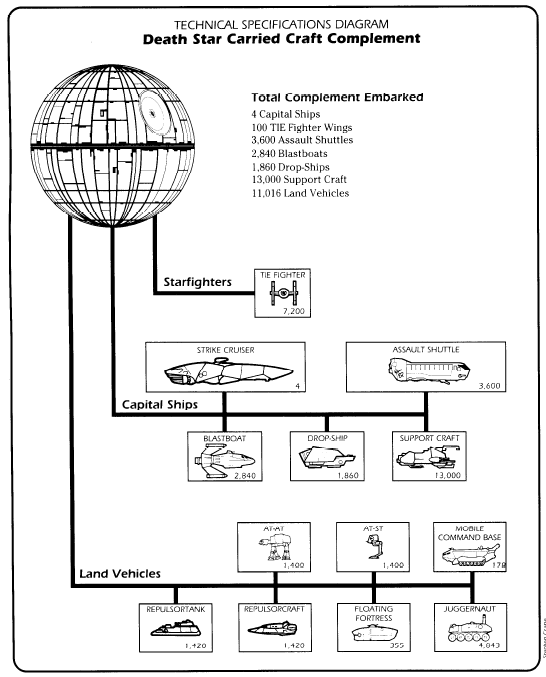
\includegraphics[width=\linewidth]{resources/plans/deathstar-crafts.png}
	\caption{\texttt{deathstar-crafts.png}}
	\label{fig:deathstar-crafts}
\end{figure}

\begin{figure}[H]
	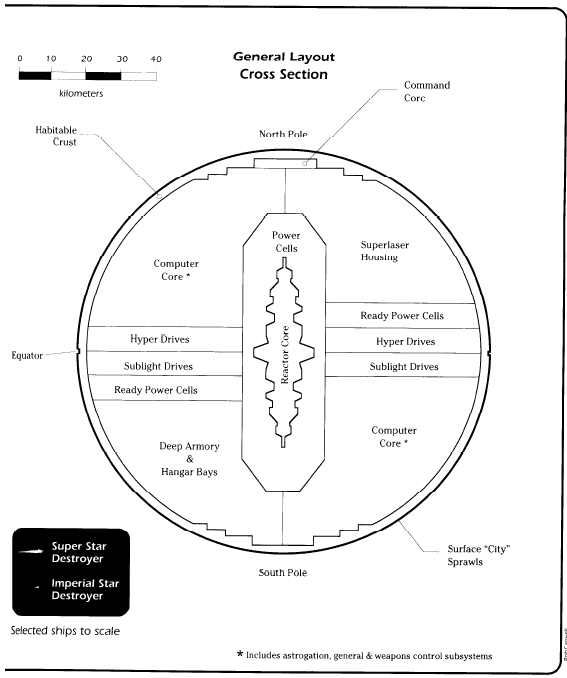
\includegraphics[width=\linewidth]{resources/plans/deathstar-cross-section.png}
	\caption{\texttt{deathstar-cross-section.png}}
	\label{fig:deathstar-cross-section}
\end{figure}

\begin{figure}[H]
	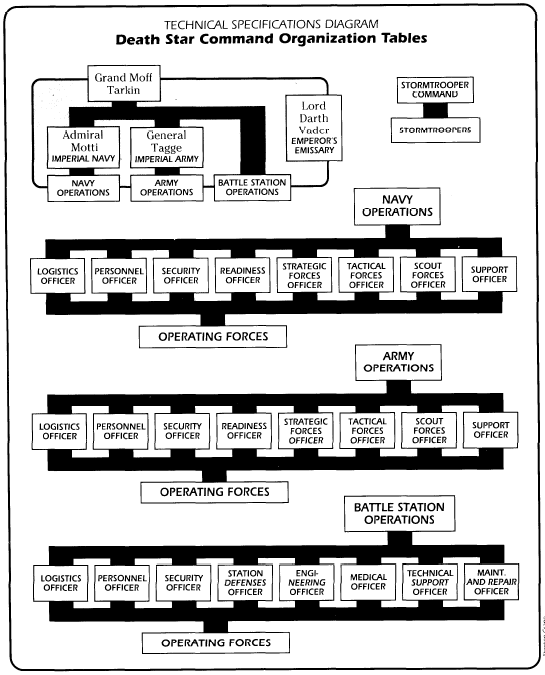
\includegraphics[width=\linewidth]{resources/plans/deathstar-operations.png}
	\caption{\texttt{deathstar-operations.png}}
	\label{fig:deathstar-operations}
\end{figure}

\begin{figure}[H]
	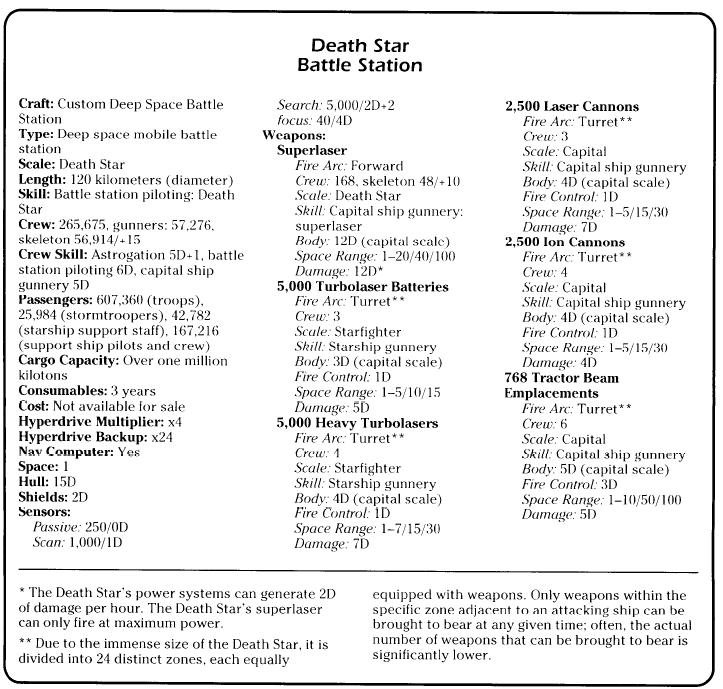
\includegraphics[width=\linewidth]{resources/plans/deathstar-summary.png}
	\caption{\texttt{deathstar-summary.png}}
	\label{fig:deathstar-summary}
\end{figure}

\begin{figure}[H]
	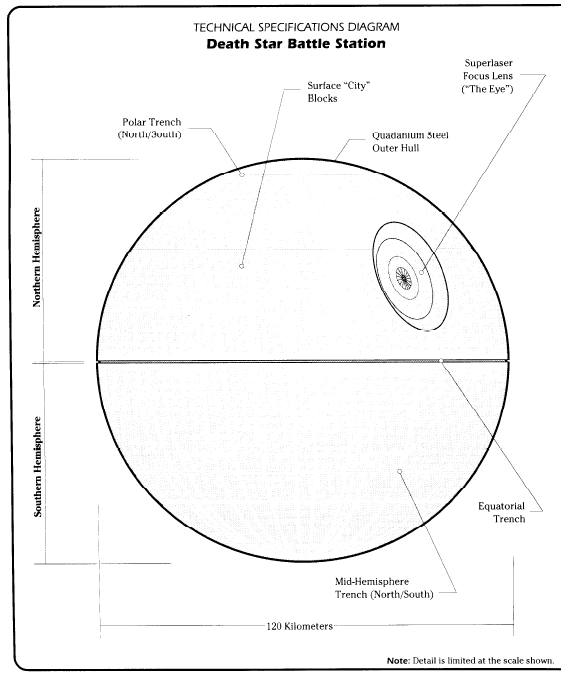
\includegraphics[width=\linewidth]{resources/plans/deathstar-technical-specs-diagram.png}
	\caption{\texttt{deathstar-techincal-specs-diagram.png}}
	\label{fig:deathstar-technical-specs-diagram}
\end{figure}

\paragraph{}
The two images below, containing information about Rebel spacerafts, were found in the server directory \texttt{/home/general\_veers/rebel-information}.

\begin{figure}[H]
	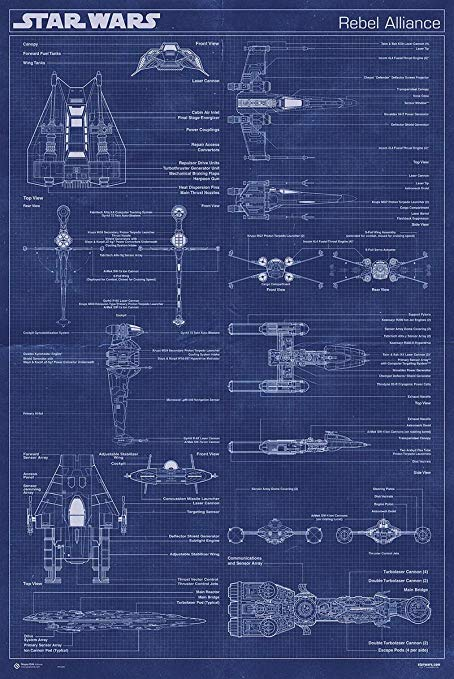
\includegraphics[width=\linewidth]{resources/plans/rebel-alliance-fleet-1.jpg}
	\caption{\texttt{rebel-alliance-fleet-1.jpg}}
	\label{fig:rebel-alliance-fleet-1}
\end{figure}

\begin{figure}[H]
	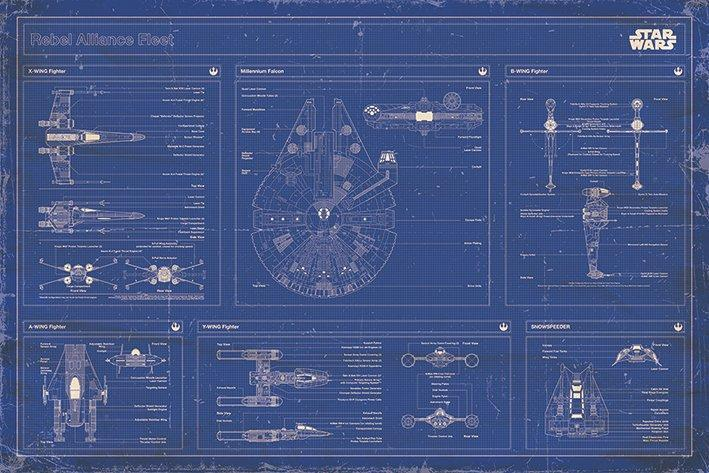
\includegraphics[width=\linewidth]{resources/plans/rebel-alliance-fleet-2.jpg}
	\caption{\texttt{rebel-alliance-fleet-2.jpg}}
	\label{fig:rebel-alliance-fleet-2}
\end{figure}

\paragraph{}
It is my firm belief that the image below will be of great value to the Rebel Alliance. It was located in the server directory \texttt{/home/darth\_sidious}.

\begin{figure}[H]
	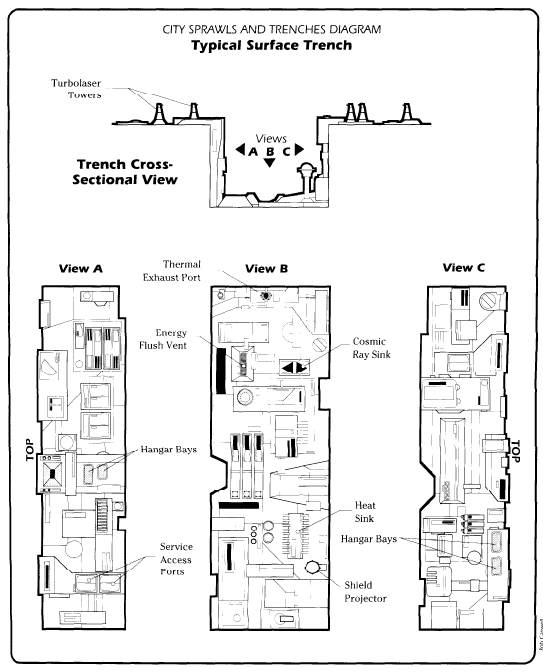
\includegraphics[width=\linewidth]{resources/plans/death-star-weakness.png}
	\caption{\texttt{death-star-weakness.png}}
	\label{fig:death-star-weakness}
\end{figure}

\paragraph{}
I was also able to recover the following photograph. It appears to be from the meeting in which the Death Star was first designed and was located in the server directoy \texttt{/home/darth\_vader}.

\begin{figure}[H]
	
\includegraphics[width=\linewidth]{resources/plans/i-love-my-death-star.jpg}
	\caption{\texttt{i-love-my-death-star.jpg}}
	\label{fig:i-love-my-death-star}
\end{figure}

\newpage

\section{Security Recommendations}
\paragraph{}
Lorem ipsum.

\end{document}
